%% Included in decks: slidemage-manual, slidemage-manual-copy
%%

%% Translation of: 1pf-EN-One-Look-Several-Institutions
%%

% SlideMage manual, chapter "The big picture": templates. The four crops are
% the same slide (1wa) compiled under each template (the MCI and Innsbruck
% templates are not part of SlideMage; the crops were made once in a project
% that has them). The color strip is live: it shows the palette of the
% template this deck uses.
\providecommand{\templatecrop}[2]{% image, caption
	\begin{tabular}[t]{@{}c@{}}
		{\setlength{\fboxsep}{0pt}\setlength{\fboxrule}{0.4pt}%
		\fcolorbox{c_primary_gray}{white}{#1}}\\[-1pt]
		{\scriptsize #2}
	\end{tabular}}
\begin{standardframe}{Ein Blick, mehrere Institutionen}
	\small
	Wie eine Folie aussieht -- Farben, Logo, Titelleiste, Fußzeile -- legt ein
	\emph{Template} fest, nicht die Folie selbst. Ein Foliensatz nennt sein Template
	nur einmal, daher erscheint dieselbe Folie in jedem Foliensatz in einem anderen
	Design -- unten eine Folie dieses Handbuchs unter vier Templates.
	\par\medskip
	\begin{columns}[T,onlytextwidth]
		\begin{column}{0.53\linewidth}
			\templatecrop{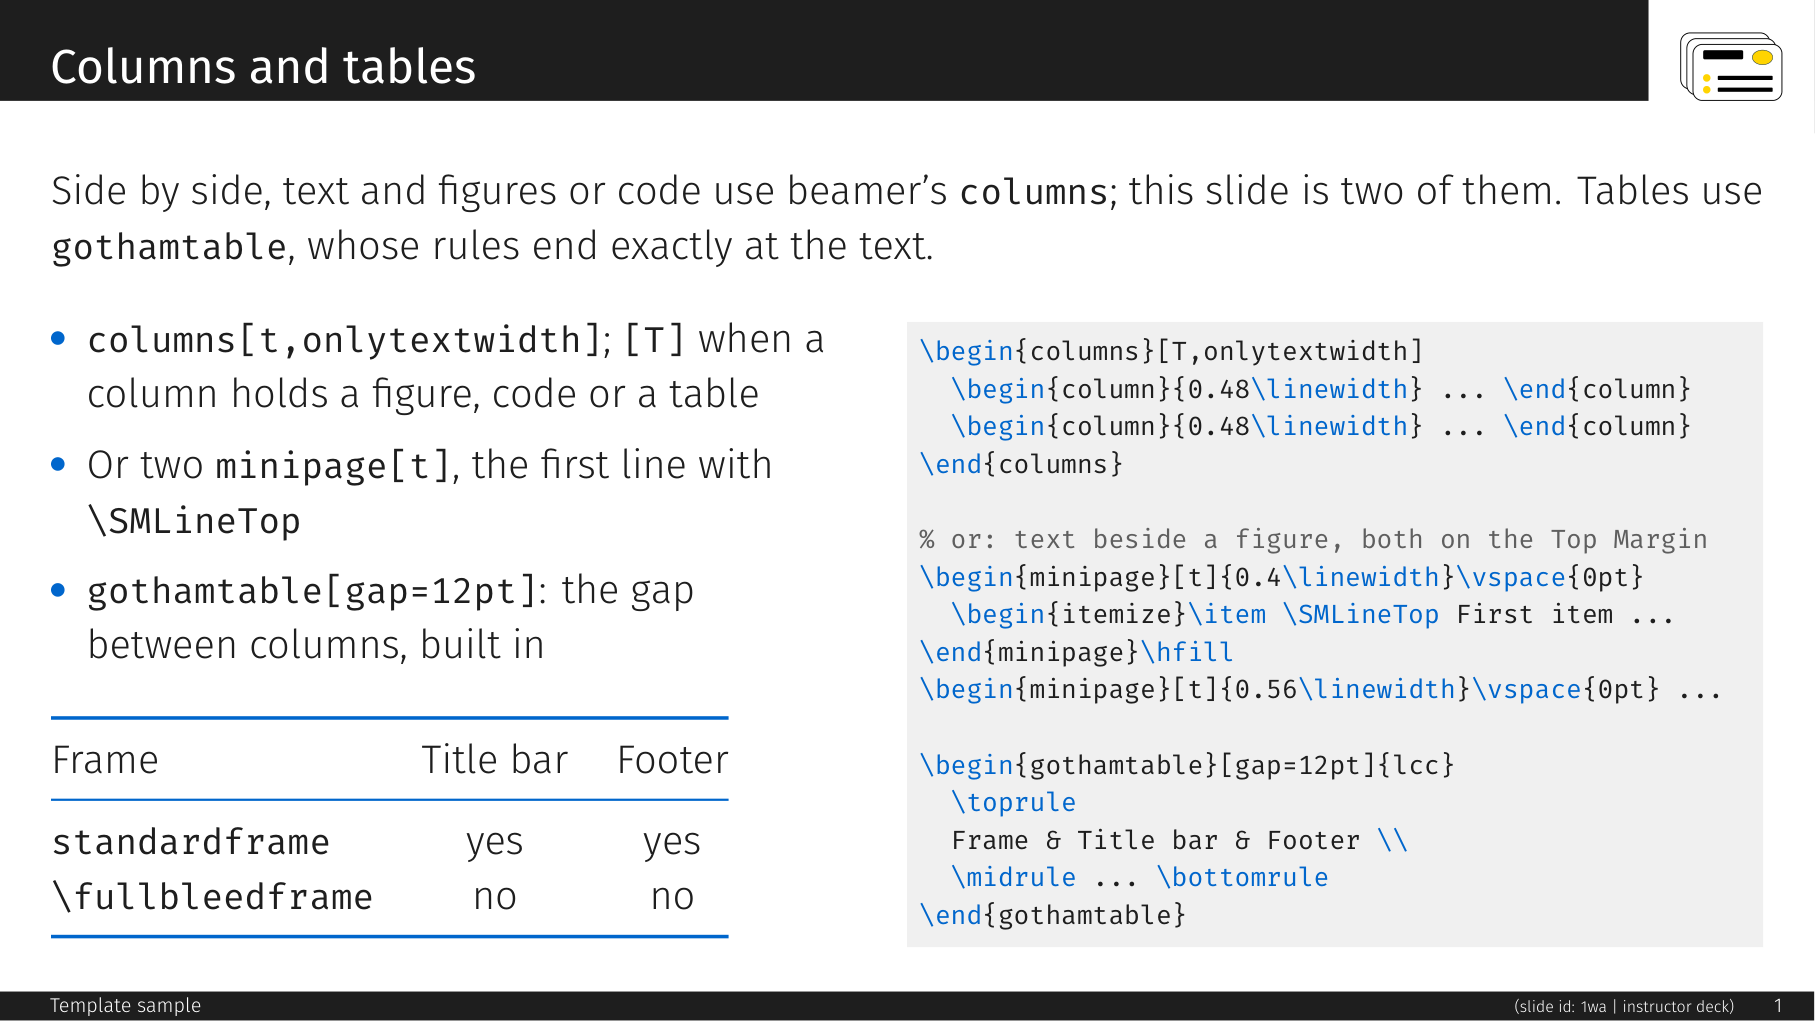
\includegraphics[width=103pt]{media/screenshot-slide-template-slidemage.png}}{SlideMage} \hspace{2pt}
			\templatecrop{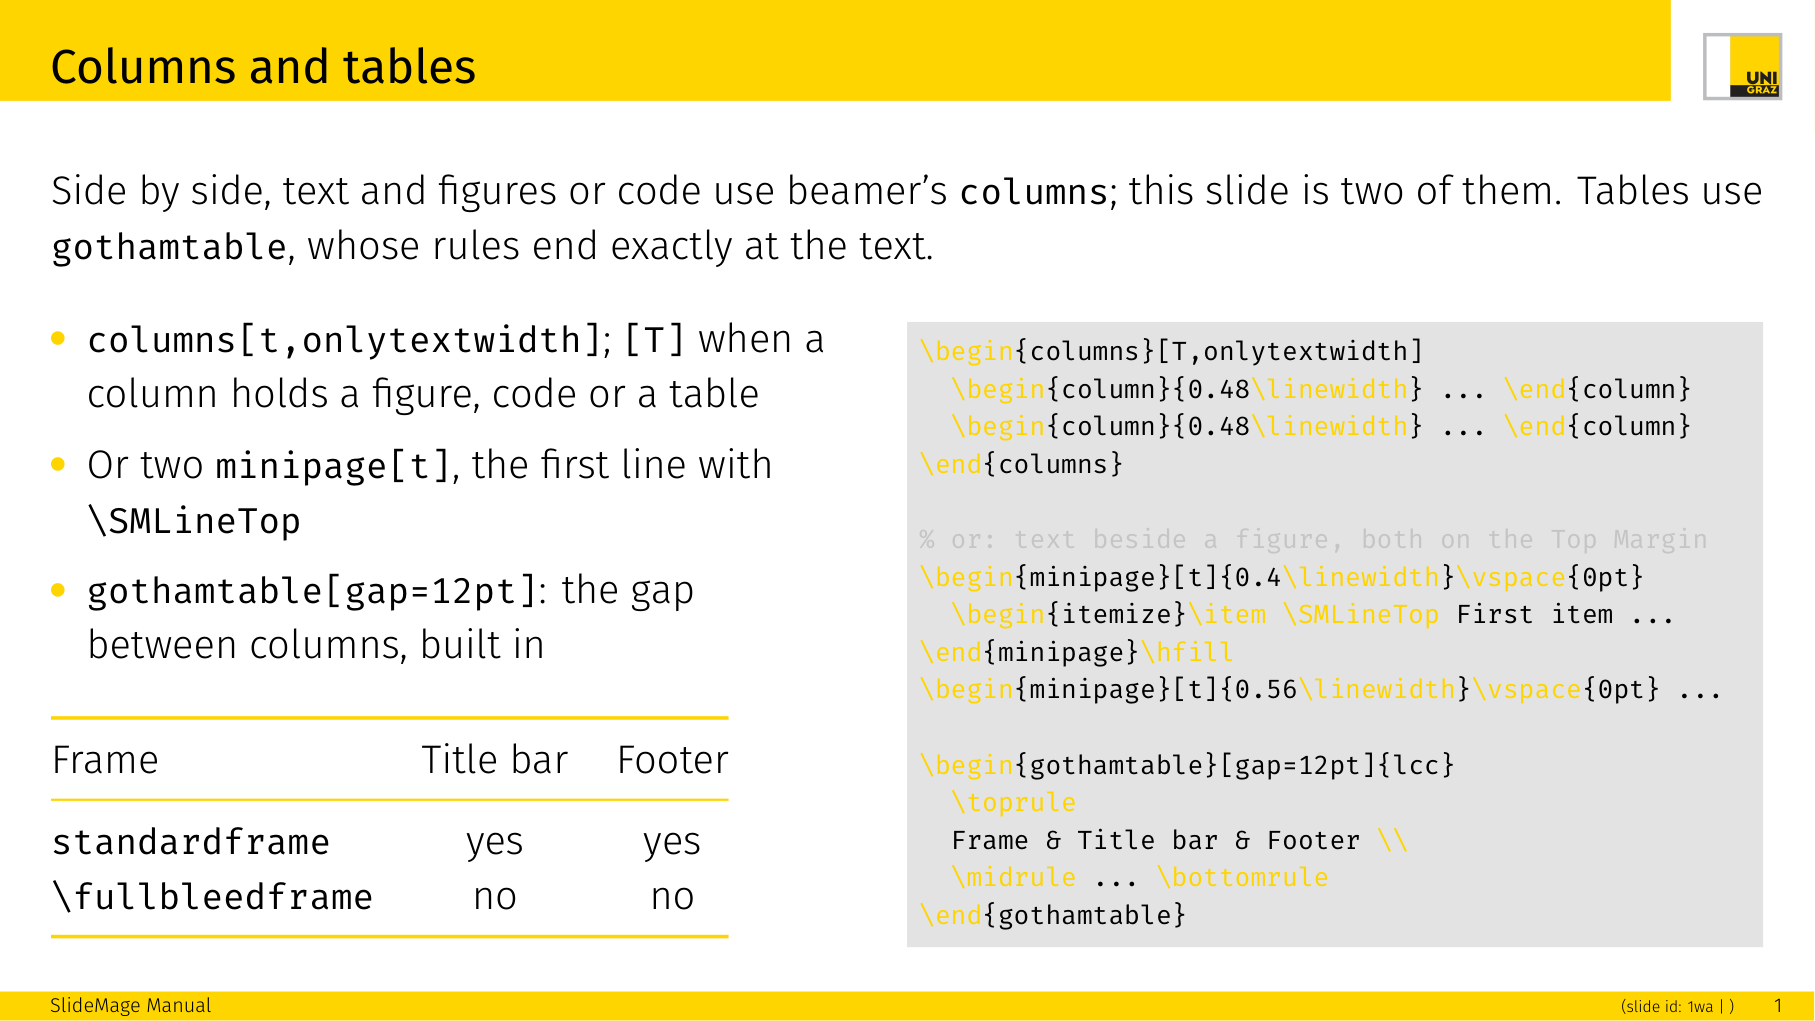
\includegraphics[width=103pt]{media/screenshot-slide-template-uni-graz.png}}{Universität Graz}\\[3pt]
			\templatecrop{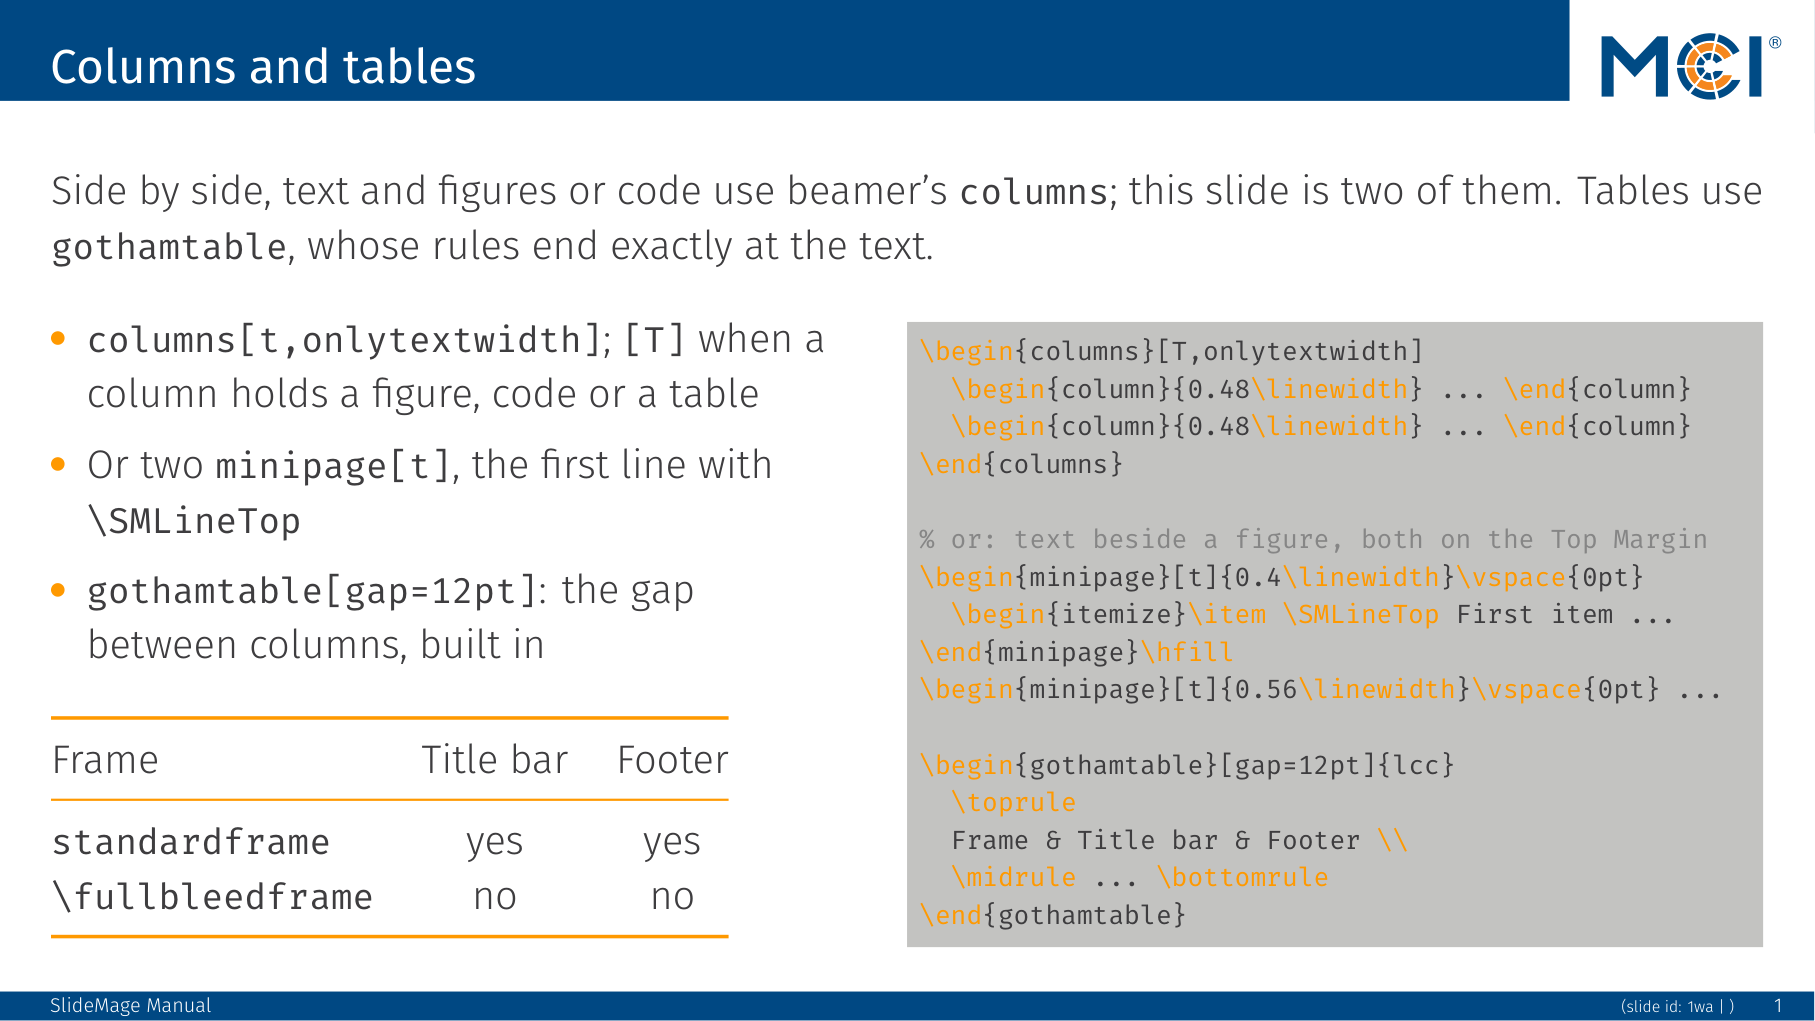
\includegraphics[width=103pt]{media/screenshot-slide-template-mci.png}}{MCI} \hspace{2pt}
			\templatecrop{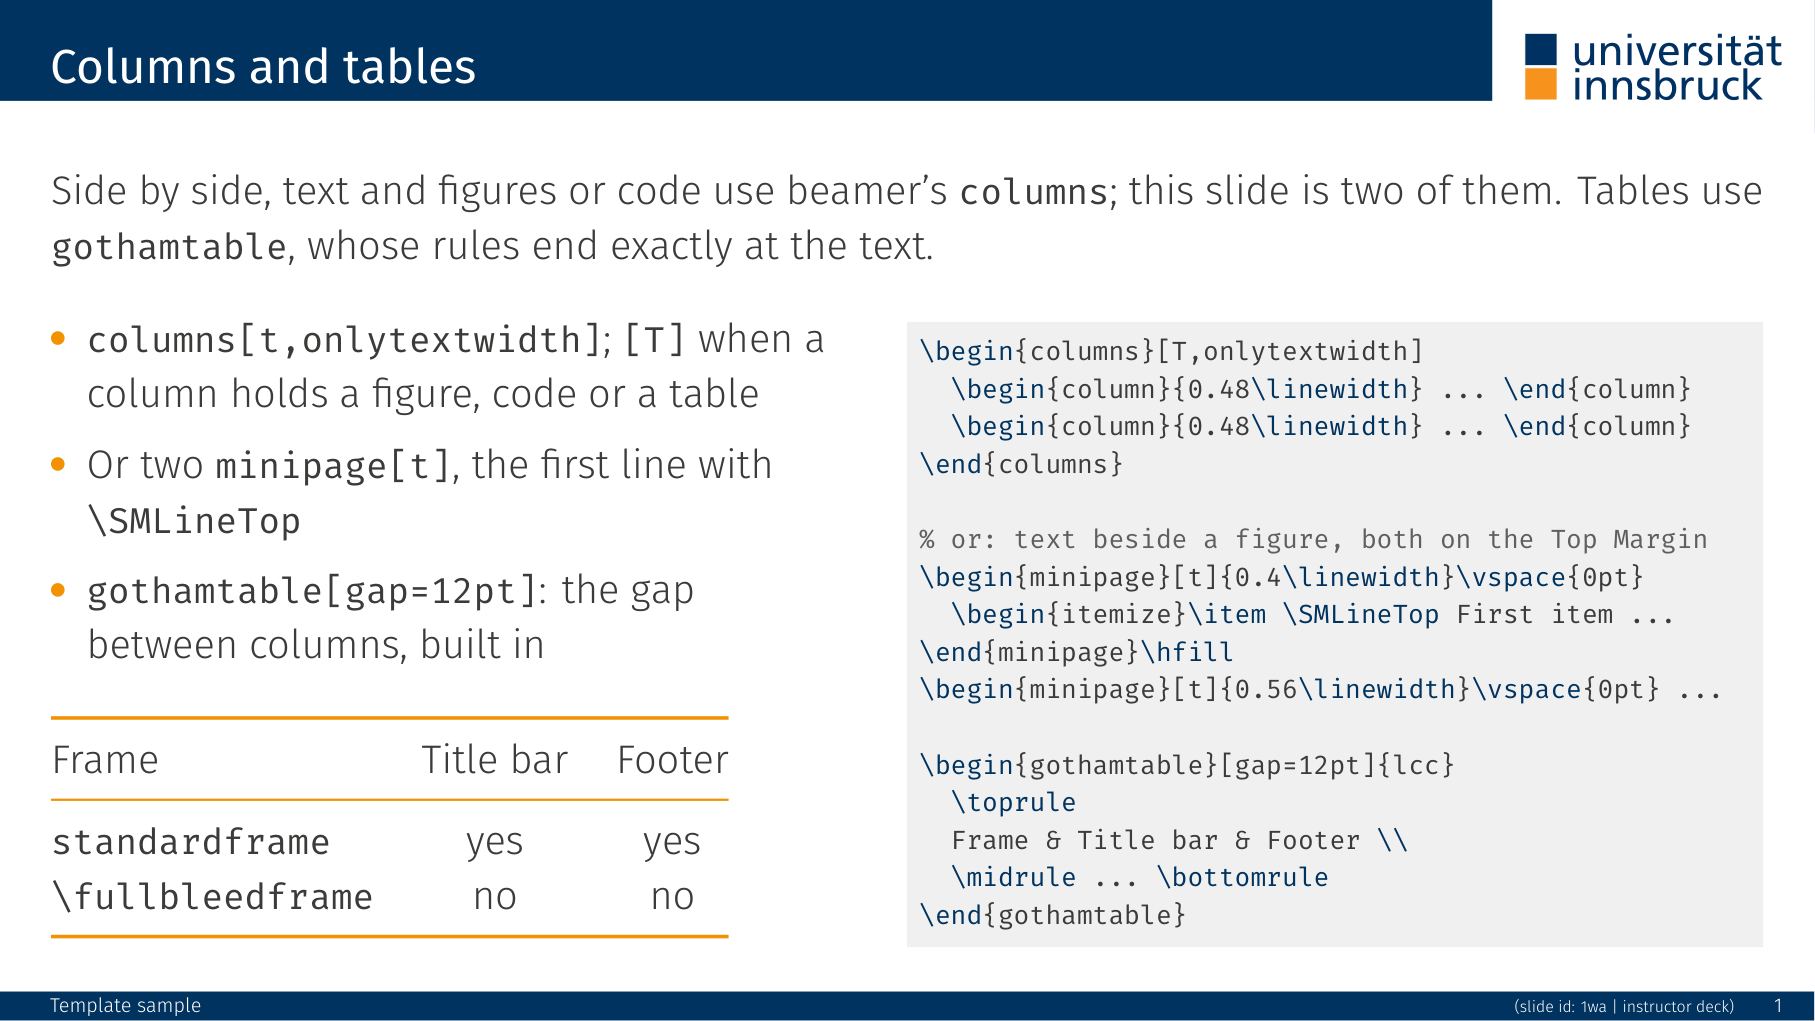
\includegraphics[width=103pt]{media/screenshot-slide-template-uni-ibk.png}}{Universität Innsbruck}
		\end{column}
		\begin{column}{0.44\linewidth}
			\shrinklists{1}
			\begin{itemize}
				\item Ein Template ist eine kleine Datei, \SMCode{SlideMage\_template\_<name>.tex}
				\item SlideMage bringt ein eigenes mit; für Ihre Institution kopieren Sie es und ändern Farben und Logo
			\end{itemize}
%			\smallskip
%			\begin{tikzpicture}[x=9.5pt, y=9.5pt]
%				\foreach \c [count=\i from 0] in {c_primary_dark, c_primary_highlight, c_primary_gray, c_primary_white, c_secondary_violet, c_tertiary_violet, c_secondary_blue, c_tertiary_blue, c_secondary_green, c_tertiary_green, c_secondary_red, c_tertiary_red, c_secondary_orange, c_tertiary_orange, c_secondary_yellow, c_tertiary_yellow, c_tertiary_gray, c_custom_gray, c_custom_red, c_custom_green, c_custom_brown}%
%					\fill[\c, draw=c_primary_gray, line width=0.2pt] ({mod(\i,11)},{-floor(\i/11)}) rectangle ++(0.85,0.85);
%			\end{tikzpicture}
		\end{column}
	\end{columns}
\end{standardframe}
